\documentclass[a4paper,notitlepage]{article}
\usepackage{ssn-format}
\title{Samples of collision cases}
\author{Atsushi Shimono}
%\date{2016--05--18}
\begin{document}

\drafttrue
\SSNID{00026}
\SSNREV{001}
\SSNCATEGORY{ICS}
\SSNChangeRecord{
}
\SSNReference{(none)}
\SSNAttachment{(none)}
\SSNWritten{Atsushi Shimono}

\ssnhead

\begin{abstract}
(TBW)
\end{abstract}

Currently, this document is just to show collision cases in PDF, 
using drawings over PostScript templates. 

References are:
\begin{description}
  \item[red dot lines] connection among center of Cobras
  \item[green dots] center of Cobras
  \item[blue dot lines] outermost radius of Cobra fiber patrol area
  \item[light blue dot lines] outermost radius of Cobra fiber arm
\end{description}


\begin{figure}[htb]
  \begin{center}
    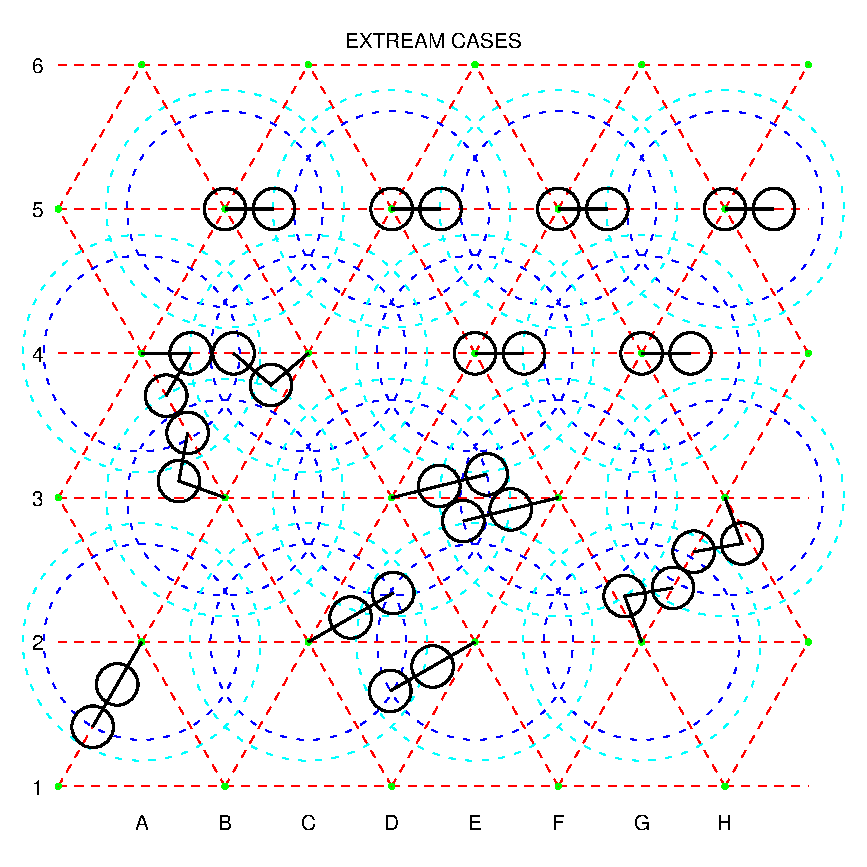
\includegraphics{extream.eps}
  \end{center}
  \caption{Extream cases}
  \label{fig:extream}
\end{figure}

Figure.~\ref{fig:extream} shows extream cases:
\begin{description}
  \item[A2] $\phi$ at 180 degree
  \item[C2, E2] Rare case of fiber at overlapped region among three Cobras
  \item[G2, H3] Two fiber tips collides with $\phi$ at 79.33 degree
  \item[D3, F3] Two Cobras can share overlapped region but in rare cases
  \item[B3, A4, C4] Fiber arm can pass Cobra 1st stage with $\phi$ at 99.5 degree
\end{description}

\begin{figure}[htb]
  \begin{center}
    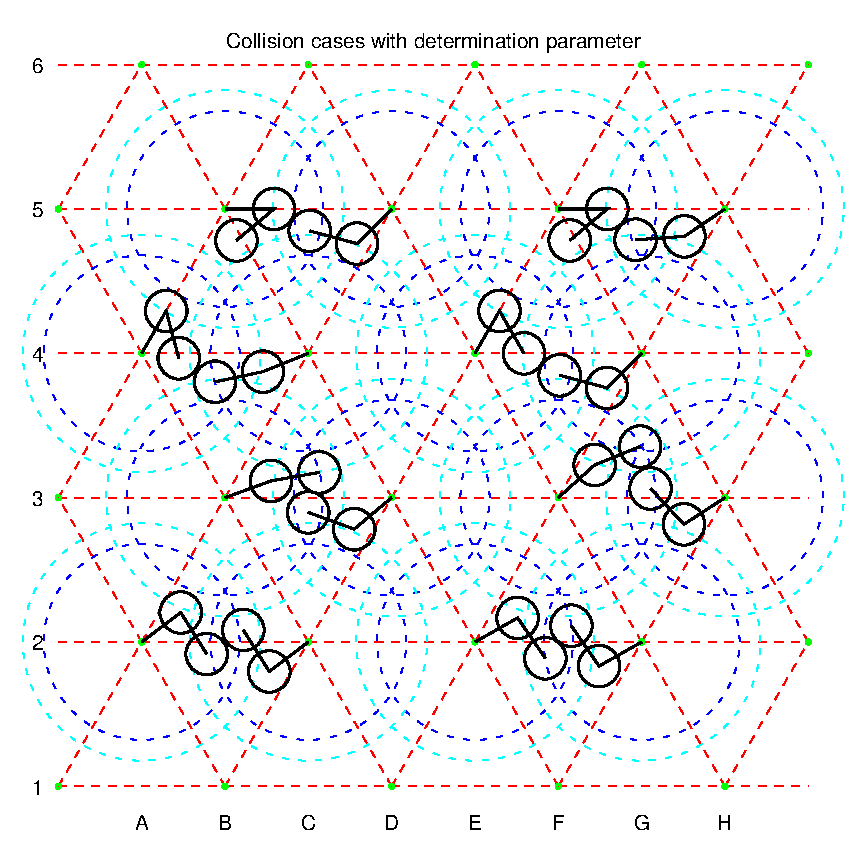
\includegraphics{cases.eps}
  \end{center}
  \caption{Collision cases}
  \label{fig:cases}
\end{figure}

Figure.~\ref{fig:cases} shows 8 collision cases with different parameter sets. 
Rows 2,3,4 show collision between two fiber tips, row 5 shows between fiber tip 
and Cobra 1st stage. 

\begin{description}
  \item[A2, C2] Both $\phi$ at 85 degree, slightly closer than pass by at 79.33 degree
  \item[E2, G2] Both $\phi$ at 95 degree, closer than A2-C2
  \item[B3, D3] $\phi$ at 170 and 120 degree, 'T' shaped collision with fiber tip nearly colliding to 1st stage of another one
  \item[F3, H3] $\phi$ at 160 and 100 degree, 'T' shaped collision between two fiber tips
  \item[A4, C4] $\phi$ at 45 and 170 degree
  \item[E4, G4] $\phi$ at 60 and 120 degree
  \item[B5, D5] $\phi$ at 40 and 120 degree, slight collision between fiber tip and 1st stage
  \item[F5, H5] $\phi$ at 40 and 150 degree, closer than B5-D5
\end{description}


\end{document}

